\documentclass[a4paper,12pt]{article}
\usepackage[a4paper,top=1.3cm,bottom=2cm,left=1.5cm,right=1.5cm,marginparwidth=0.75cm]{geometry}
\usepackage{setspace}
\usepackage{array}
\usepackage{cmap}					
\usepackage{mathtext} 				
\usepackage[T2A]{fontenc}			
\usepackage[utf8]{inputenc}			
\usepackage[english,russian]{babel}
\usepackage{multirow}
\usepackage{graphicx}
\usepackage{wrapfig}
\usepackage{tabularx}
\usepackage{bm}
\usepackage{float}
\usepackage{longtable}
% \usepackage{upgreek}
\usepackage{hyperref}
\usepackage{textcomp}
\hypersetup{pdfstartview=FitH,  linkcolor=linkcolor,urlcolor=urlcolor, colorlinks=true}
\hypersetup{
    colorlinks=true,
    linkcolor=blue,
    filecolor=magenta,      
    urlcolor=cyan,
    pdftitle={Overleaf Example},
    pdfpagemode=FullScreen,
    }
\usepackage[rgb]{xcolor}
\usepackage{amsmath,amsfonts,amssymb,amsthm,mathtools} 
\usepackage{icomma} 
\mathtoolsset{showonlyrefs=true}
\usepackage{euscript}
\usepackage{mathrsfs}
\usepackage{ dsfont }
\linespread{1.25} 
\date{}
\DeclareMathOperator{\rg}{rg}
\DeclareMathOperator{\im}{Im}
\DeclareMathOperator{\mker}{Ker}
\DeclareMathOperator{\tr}{tr}
\DeclareMathOperator{\det}{det}
\DeclareMathOperator{\d}{d}


\graphicspath{{Images/}}

\begin{document}

\begin{titlepage}
	\begin{center}
		\large 	Московский физико-технический институт \\
		\vspace{0.2cm}
		
		\vspace{4.5cm}
		\LARGE \textbf{Вопрос по выбору} \\ \vspace{0.2cm}
		\large (Общая физика: квантовая физика) \\ \vspace{0.2cm}
		\LARGE \textbf{СОЛНЦЕ И ЕГО ТЕМПЕРАТУРА}
	\end{center}
	\vspace{2.3cm} \large
	
	\begin{center}
		Работу выполнили: \\
        \textbf{Лазарь Владислав}, группа Б01-207
        \vspace{0.3cm}
        
        \textbf{Шибина Полина}, группа Б01-209

	\end{center}
	\begin{center} \vspace{100mm}
		г. Долгопрудный \\
		 Январь, 2025 год
	\end{center}
\end{titlepage}

% \section*{Цель работы}
% Оценка температуры всех слоёв Солнца.

\section*{Почему Солнце светит?}
 В конце XIX века Кельвин и Гельмгольц предложили гипотезу для объяснения источника энергии Солнца. Поскольку ядерные процессы были на тот момент неизвестны, главным кандидатом для объяснения этой энергии стало гравитационное сжатие. Гипотеза представляет собой процесс, который происходит, когда поверхность звезды или планеты остывает. Охлаждение приводит к снижению внутреннего давления, в результате чего звезда или планета сжимается. Это сжатие, в свою очередь, нагревает ядро звезды/планеты. 

 Чтобы вычислить общее количество энергии, которое будет выпущено Солнцем в таком механизме (при условии однородной плотности), оно было аппроксимировано идеальной сферой, состоящей из концентрических оболочек. Тогда полную потенциальную энергию можно было бы найти как интеграл по всем оболочкам от центра до внешнего радиуса. Итак, полная потенциальная энергия:
 \[
 U = \frac{Gm_1m_2}{r},
 \]
где $G = 6.67 \cdot 10^{-11} \frac{H \cdot \text{м}^2}{\text{кг}^2}$ --- гравитационная постоянная, а две массы в данном случае --- это масса тонкой оболочки шириной $dr$ и масса, заключённая в пределах радиуса r. Тогда:

\[
U = -G\int_0^R\frac{m(r)\cdot 4\pi r^2\rho}{r}dr, 
\]

\noindentгде R --- внешний радиус сферы, а $m(r)$ --- масса, заключённая в пределах радиуса r, тогда:

\[
U = -G\int_0^R\frac{4\pi r^3\rho\cdot 4\pi r^2\rho}{3r}dr = -\frac{16}{15}G\pi^2\rho^2R^5 = -\frac{3}{5}\frac{G M^2}{R}
\]


Согласно теореме Вириала, полная энергия гравитационно-связанных систем, находящихся в равновесии, равна половине усредненной по времени потенциальной энергии: 

\[
U_r = \frac{|\langle U \rangle|}{2} = \frac{3}{10}\frac{G M^2}{R}
\]

Хотя плотность нашей звезды не является однородной, можно получить приблизительное представление о порядке величины ожидаемого возраста нашей звезды, исходя из рассуждений Кельвина и Гельмгольца. Считаем известными нам светимость, массу и радиус Солнца\\ $L_\odot = 3.846 \cdot 10^{26} \text{ Вт, } M_{\text{С}} = 1.9885 \cdot 10^{30} \text{ кг, } R_{\text{С}} = 6.96 \cdot 10^8 \text{ м}$, тогда:

\[
\tau = \frac{U_r}{L_\odot} \approx \frac{1.1\cdot 10^{41} \text{ Дж}}{3.828\cdot 10^{26} \text{ Вт}} = 2.874 \cdot 10^{14} \text{ с} \approx 8\,900\,000 \text{ лет}.
\]

И это значение расходится на несколько порядков с геологическими и биологическими наблюдениями на Земле $(\approx 4\,600\,000\,000 \text{ лет})$.

В 1930-х годах Ханс Бете выяснил детали того, как происходит ядерный синтез внутри Солнца. Он установил, что в недрах Солнца атомы водорода сливаются в гелий, высвобождая при этом огромное количество энергии. 

Превращение водорода в гелий идёт через ряд промежуточных реакций. Оно может выполняться двумя путями:
\begin{enumerate}
\item В протонно-протонной(pp) цепочке реакций, или водородном цикле;
\item В углеродно-азотном или углеродном цикле.
\end{enumerate}

Для Солнца преобладающим является водородный цикл, так как в звёздах главной последовательности (к ним относится Солнце) энерговыделение происходит главным образом за счёт превращения водорода в гелий. Рассмотрим подробнее протонно-протонную цепочку.

\begin{figure}[H]
		\centering
		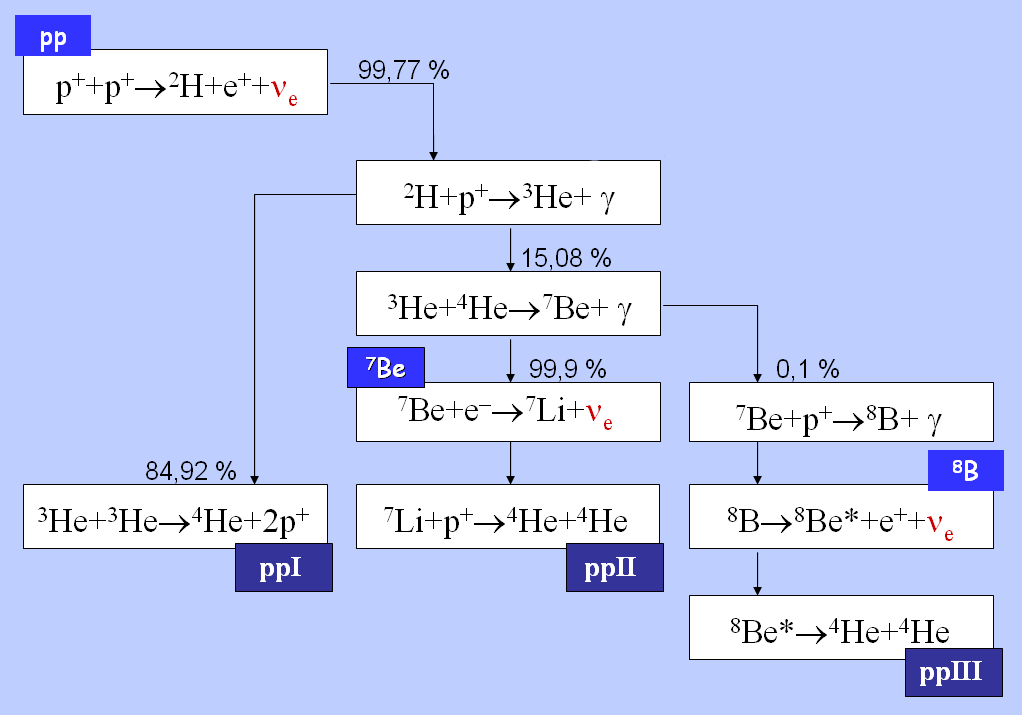
\includegraphics[width=150mm]{Images/Proton_proton_cycle.png}
        \caption{Схема протонно-протонной цепочки}
\end{figure}

\begin{table}[H]
    \centering
    \renewcommand{\arraystretch}{1.5} % Увеличение межстрочного расстояния в таблице
    \begin{tabular}{|c|c|c|} 
        \hline
        Реакция & Энерговыделение, МэВ & Среднее время реакции \\ \hline
        $p + p \rightarrow d + e^+ + \nu_e$ & $2 \cdot 0.164 + (2 \cdot 0.257)$ & $1.4 \cdot 10^{10} \text{лет}$ \\ \hline
        $e^+ + e^- \rightarrow 2\gamma$ & $2 \cdot 1.02 $ & --- \\ \hline
        $p + d \rightarrow \mathrm{{}^{3}He} + \gamma$ & $2 \cdot 5.49$ & 5.7 с \\ \hline
        $\mathrm{{}^{3}He} + \mathrm{{}^{3}He} \rightarrow \mathrm{{}^{4}He} + 2p$ & 12.85 & $10^6$ лет \\ \hline
        $\text{Итого: } 4p \rightarrow \mathrm{{}^{4}He} + 2e^+ + 2\nu$  & 26.21 + (0.514) &  \\ \hline
    \end{tabular}
    \caption{Водородный цикл}
\end{table}

Водородный цикл начинается с реакции между двумя протонами, в результате которой образуется дейтрон, позитрон и нейтрино. Эта реакция вызывается слабыми взаимодействиями, а потому идёт чрезвычайно медленно. Позитрон немедленно аннигилирует с электроном, а дейтрон очень быстро вступает в реакцию с одним из ближайших протонов с образованием ядра $\mathrm{{}^{3}He}$. Далее возможны три ветви ядерных реакций.

Первая ветвь --- это реакция между двумя ядрами $\mathrm{{}^{3}He}$. Но так как в первых трёх реакциях ядро $\mathrm{{}^{3}He}$ получается только один раз, то в рассматриваемый вариант полного водородного цикла эта реакция должна входить дважды, что и отмечено множителем \textbf{2} во втором столбце таблицы. В итоге цикла 4 протона превращаются в ядро $\mathrm{{}^{4}He}$, два позитрона и два нейтрино. В таблице приведено энерговыделение в соответствующих реакциях, а также примерное среднее время каждой реакции, рассчитанное для условий в центре Солнца. В скобках указана доля выделяющейся энергии, безвозвратно уносимая нейтрино.

При достаточно больших концентрациях $\mathrm{{}^{4}He}$ и температурах $T > (10$---$15)\cdot 10^6$ К в полном энерговыделении начинает преобладать вторая ветвь водородного цикла, расположенная посередине схемы. В этом варианте первые три реакции такие же, как и в предыдущем, но не повторяются дважды.

При ещё более высоких температурах преобладающим в энерговыделении является водородный цикл, расположенный справа на схеме.

Энергия, выделяемая на каждом этапе, поддерживает светимость Солнца, а нейтрино, слабо взаимодействующие с веществом, покидают ядро и все остальные слои Солнца, не подвергаясь существенным изменениям.

В 1960-х годах Рэймонд Дэвис провел первый эксперимент по измерению солнечных нейтрино в обсерватории Homestake, использовав метод хлор-аргоновой детекции:
\[
\nu_e + \mathrm{{}^{37}Cl} \rightarrow \mathrm{{}^{37}Ar} + e^{-}
\]
\[
\mathrm{{}^{37}Ar} + e^{-} \rightarrow \mathrm{{}^{37}Cl} +  \nu_e
\]

Однако наблюдаемый поток нейтрино составлял лишь около одной трети от предсказанного Стандартной солнечной моделью. Почему? Можно предпоположить следующие варианты.

\begin{itemize}
    \item Возможно ли, что Стандартная солнечная модель содержит ошибки в расчетах термоядерных реакций или солнечных условий? 
    \item Являются ли нейтрино стабильными частицами или могут изменяться в процессе распространения от ядра Солнца к Земле? Если нейтрино меняет тип по пути к Земле\\ ($\nu_e\to\nu_\mu$), оно уже не может взаимодействовать с рождением электрона. Общий поток $\nu_e+\nu_\mu$ не поменялся.
\end{itemize}

 Бруно Понтекорво за год до получения результатов эксперимента Рэймонда Дэвиса разрабатывает теорию, как именно нейтрино могут менять свой тип в вакууме. Одно из следствий --- у разных типов нейтрино должна быть разная масса.

 Обычно нейтринный поток раскладывают на разные типы: электронное ($\nu_e$), мюонное ($\nu_\mu$) и таонное ($\nu_\tau$). Если из Солнца летит поток исключительно электронных нейтрино, то это состояние (1, 0, 0) в выбранном нами базисе. Но нейтрино могут быть массивными, причем обладать разными массами. А значит можно разложить поток нейтрино и по массовым состояниям: $\nu_1, \nu_2, \nu_3$ с массами $m_1, m_2, m_3$ соответственно.

То есть, если в термоядерной реакции появилось электронное нейтрино, то появились сразу три массовых состояния (спроектировали $\nu_e$ на $\nu_1,\ \nu_2,\ \nu_3$). 

\begin{figure}[H]
		\centering
		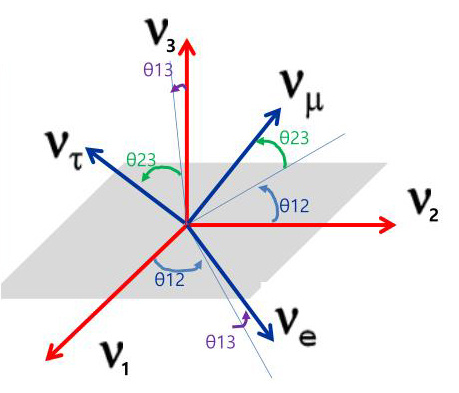
\includegraphics[width=110mm]{Images/muon_mass.jpg}
\end{figure}

Но если у этих состояний разные массы, то и энергии будут отличаться. А раз отличаются энергии, то и распространяться в пространстве они будут по-разному. На рисунке ниже показано, как именно будут эволюционировать эти три состояния во времени. 

\begin{figure}[H]
		\centering
		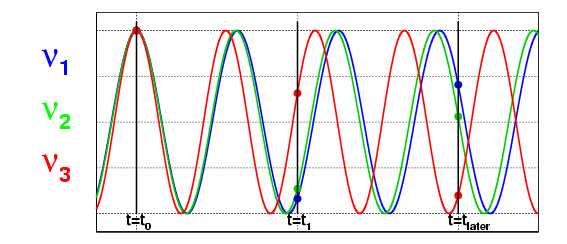
\includegraphics[width=160mm]{Images/muon_evolution.jpg}
\end{figure}

Нейтрино взаимодействуют с веществом в зависимости от типа по-разному ($e, \mu, \tau$). Поэтому, когда мы хотим посчитать, как нейтрино себя проявит, нужно спроектировать наш вектор состояния на ($\nu_e, \nu_\mu, \nu_\tau$). И таким образом получится вероятность зарегистрировать тот или иной тип нейтрино. Вот такие волны вероятности мы получим для электронного нейтрино в зависимости от пройденного расстояния:

\begin{figure}[H]
		\centering
		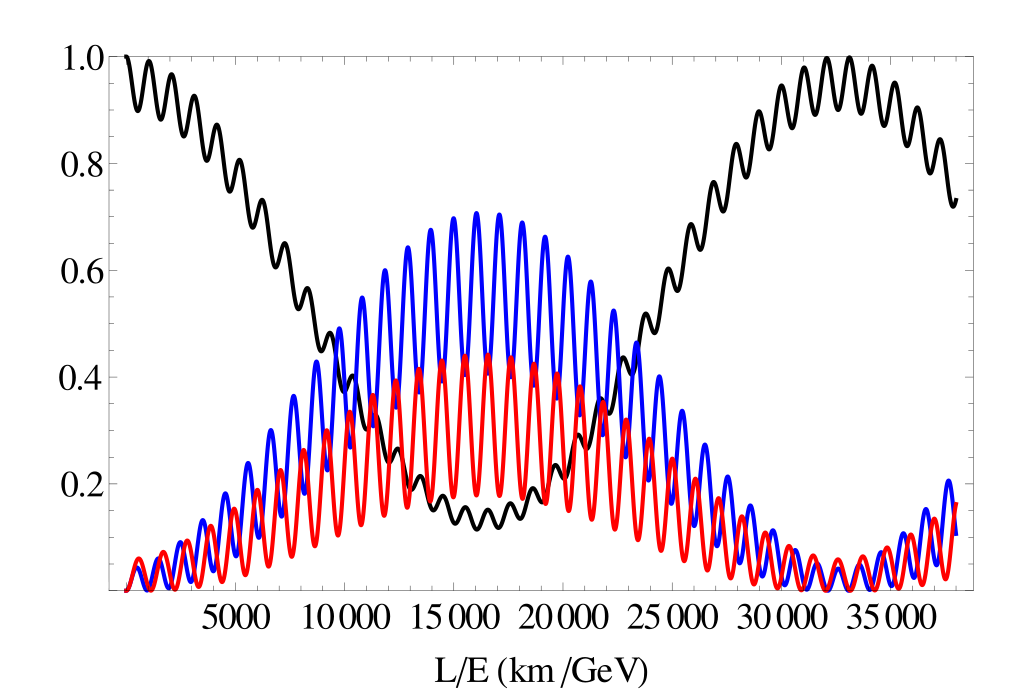
\includegraphics[width=170mm]{Images/Oscillations_electron_long.png}
        \caption{чёрная волна ($P: \nu_e \rightarrow \nu_e)$, синяя волна ($P: \nu_e \rightarrow \nu_{\mu})$, красная волна ($P: \nu_e \rightarrow \nu_{\tau}$)}
\end{figure}


\newpage
\section*{Оценка температуры хромосферы}

\begin{figure}[H]
		\centering
		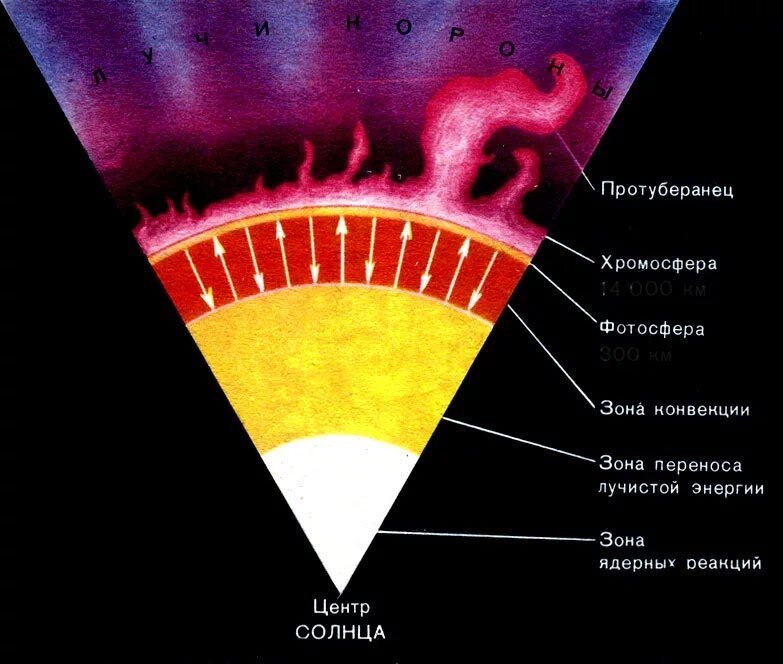
\includegraphics[width=110mm]{Images/Sun_layers.jpeg}
        \caption{Слои Солнца}
\end{figure}

Весь видимый нами свет Солнца излучается фотосферой, а в хромосфере формируется линейчатый спектр поглощения. Таким образом, изучая поглощения света, можно оценить температуру хромосферы.

Солнечный спектр --- сплошной, но перекрывается темными провалами линий поглощения. 
Рассмотрим на примере атома водорода. Атом водорода может поглощать свет только дискретными порциями, т.е. определенных частот, которые смогут перевести электрон на одну из более высоких орбиталей.

В лабораторных условиях водород дает достаточно тонкие линии излучения и поглощения, т.к. его температура и скорость его молекул достаточно низкая ($T \approx 300 \text{ К}; v = \sqrt{\frac{3k_{\text{Б}}T}{m}} \approx 1.9\ \frac{\text{км}}{\text{с}}$).

Но при высокой температуре наблюдается доплеровское уширение — это расширение спектральных линий из-за эффекта Доплера, вызванного распределением кинетических энергий молекул или атомов. В этом случае атом водорода в силу его движения с большой скоростью сможет поглощать свет близких частот.
\[
\nu = \nu_{0}\cdot \left(1 + \frac{v}{c}\right) \Rightarrow \frac{\Delta\nu}{\nu_0} = \frac{v}{c} = \frac{\Delta\lambda}{\lambda_0} \Rightarrow \lambda = \lambda_{0}\cdot \left(1 + \frac{v}{c}\right)    
\]

Таким образом, мы можем определить $v$, которая, в свою очередь, зависит от температуры. 
Для работы использовался сайт Парижской обсерватории, содержащий онлайн версию атласа солнечного спектра. Так как будем пользоваться видимым диапазоном спектра, то 
линии, на которых водород поглощает, это линии серии Бальмера.

В итоге получаем $T_{\text{ср}} = $ 12 569 К --- средняя температура хромосферы. Табличные данные варьируются от 4000 К до 18 000 К.

\begin{table}[H]
    \centering
    \renewcommand{\arraystretch}{1.5} % Увеличение межстрочного расстояния в таблице
    \begin{tabular}{|c|m{2.6cm}|m{2.6cm}|c|c|c|c|c|} 
        \hline
        $n$ & Длина волны на перегибе слева $\lambda_L$, нм & Длина волны на перегибе справа $\lambda_R$, нм & $\lambda_{min}$, нм & $\lambda_{min\_theor}$, нм & $\Delta\lambda$, нм & $v$, $\frac{\text{м}}{\text{с}}$ & $T$, K \\ \hline
        3 &\ \ \ \ \ \ 656.24 &\ \ \ \ \ \ 656.32 & 656.29 & 656.47 & 0.08 & 18 284 & 13 485 \\ \hline
        4 &\ \ \ \ \ \ 486.10 &\ \ \ \ \ \ 486.16 & 486.13 & 486.27 & 0.06 & 18 513 & 13 825 \\ \hline
        5 &\ \ \ \ \ \ 434.02 &\ \ \ \ \ \ 434.07 & 434.05 & 434.17 & 0.05 & 17 278 & 12 042 \\ \hline
        6 &\ \ \ \ \ \ 410.14 &\ \ \ \ \ \ 410.19 & 410.17 & 410.29 & 0.045 & 16 456 & 10 923 \\ \hline
    \end{tabular}
    \caption{данные с сайта Парижской обсерватории}
\end{table}


На рисунке ниже показано, как это выглядит на сайте. Рассмотрим подробнее выделенный пик, для $n = 3$.

\begin{figure}[H]
		\centering
		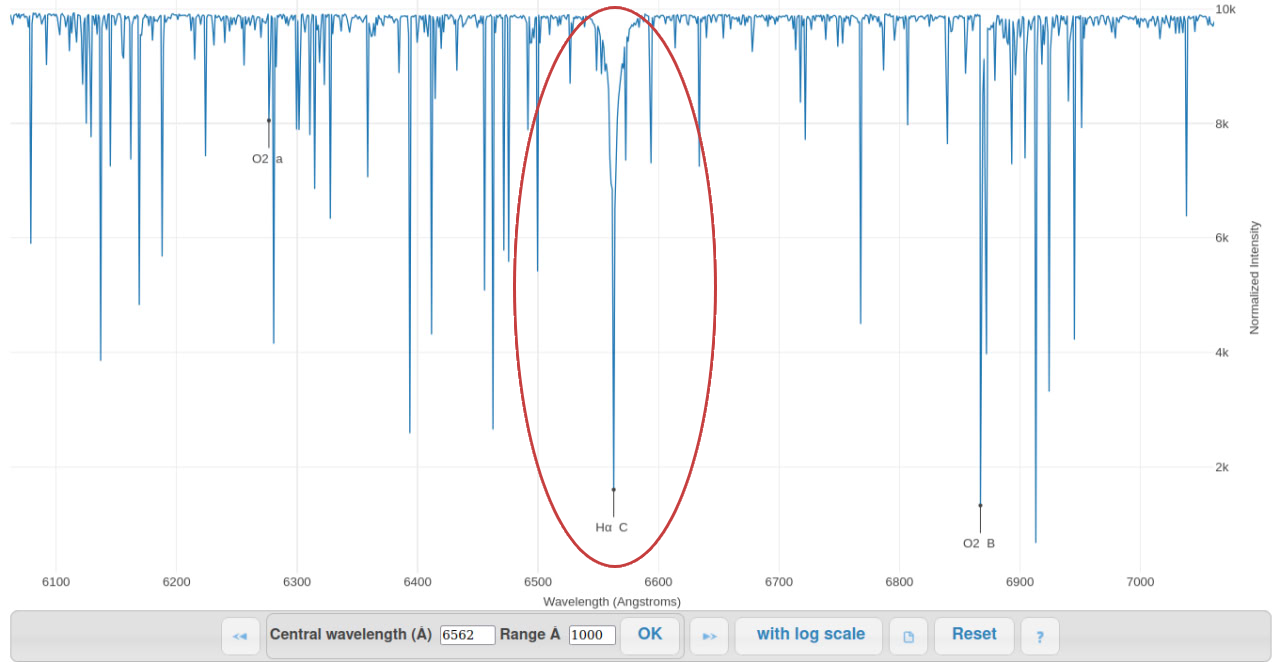
\includegraphics[width=160mm]{Images/1.png}
\end{figure}

\begin{figure}[H]
		\centering
		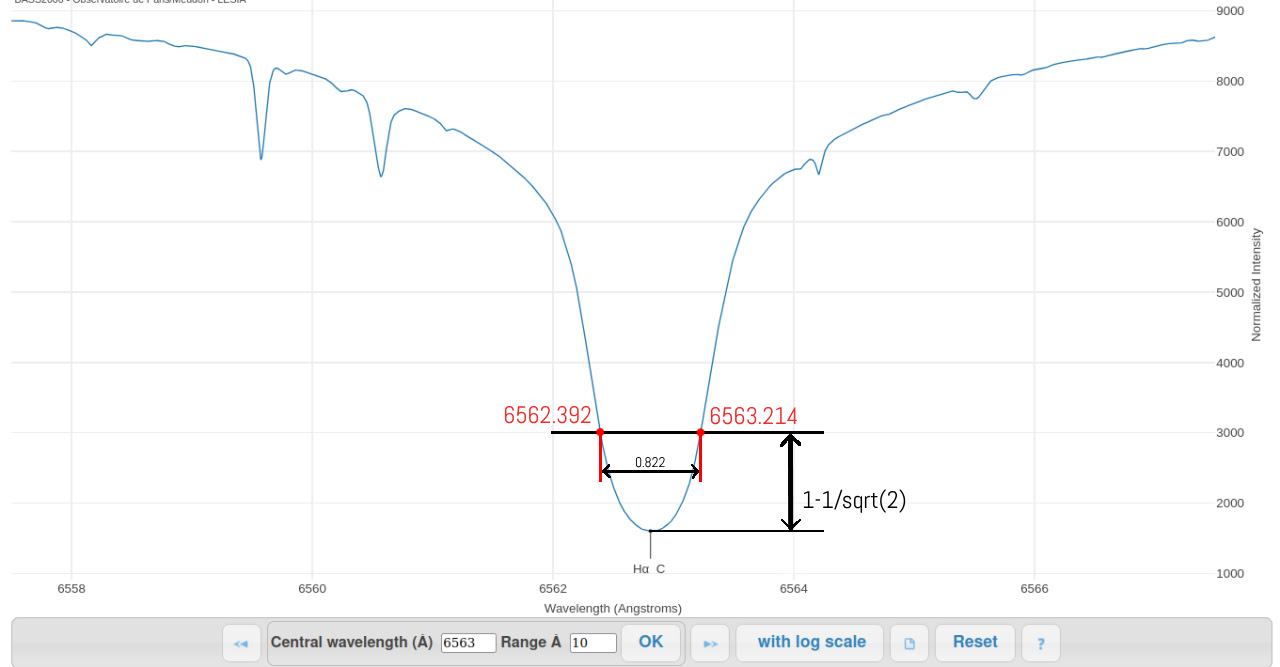
\includegraphics[width=160mm]{Images/2.png}
\end{figure}

\section*{Оценка температуры фотосферы}
Фотосфера --- это тонкий поверхностный слой Солнца, испускающий основную часть излучения в оптическом диапазоне спектра. Фотосфера существенно непрозрачна, она поглощает и затем переизлучает энергию, поступающую из недр звезды. Перенос энергии происходит конвективным путём: конвекция наблюдается как грануляция фотосферы, то есть в виде светлых горячих конвективных гранул. Гранулы представляют собой короткоживущие ячейки, в пределах которых горячее вещество Солнца (плазма) всплывает снизу вверх в центре гранулы и растекается от центра к краю. На краях гранул остывшее вещество опускается вниз в конвективную зону. Такая циркуляция происходит непрерывно.

\begin{figure}[H]
		\centering
		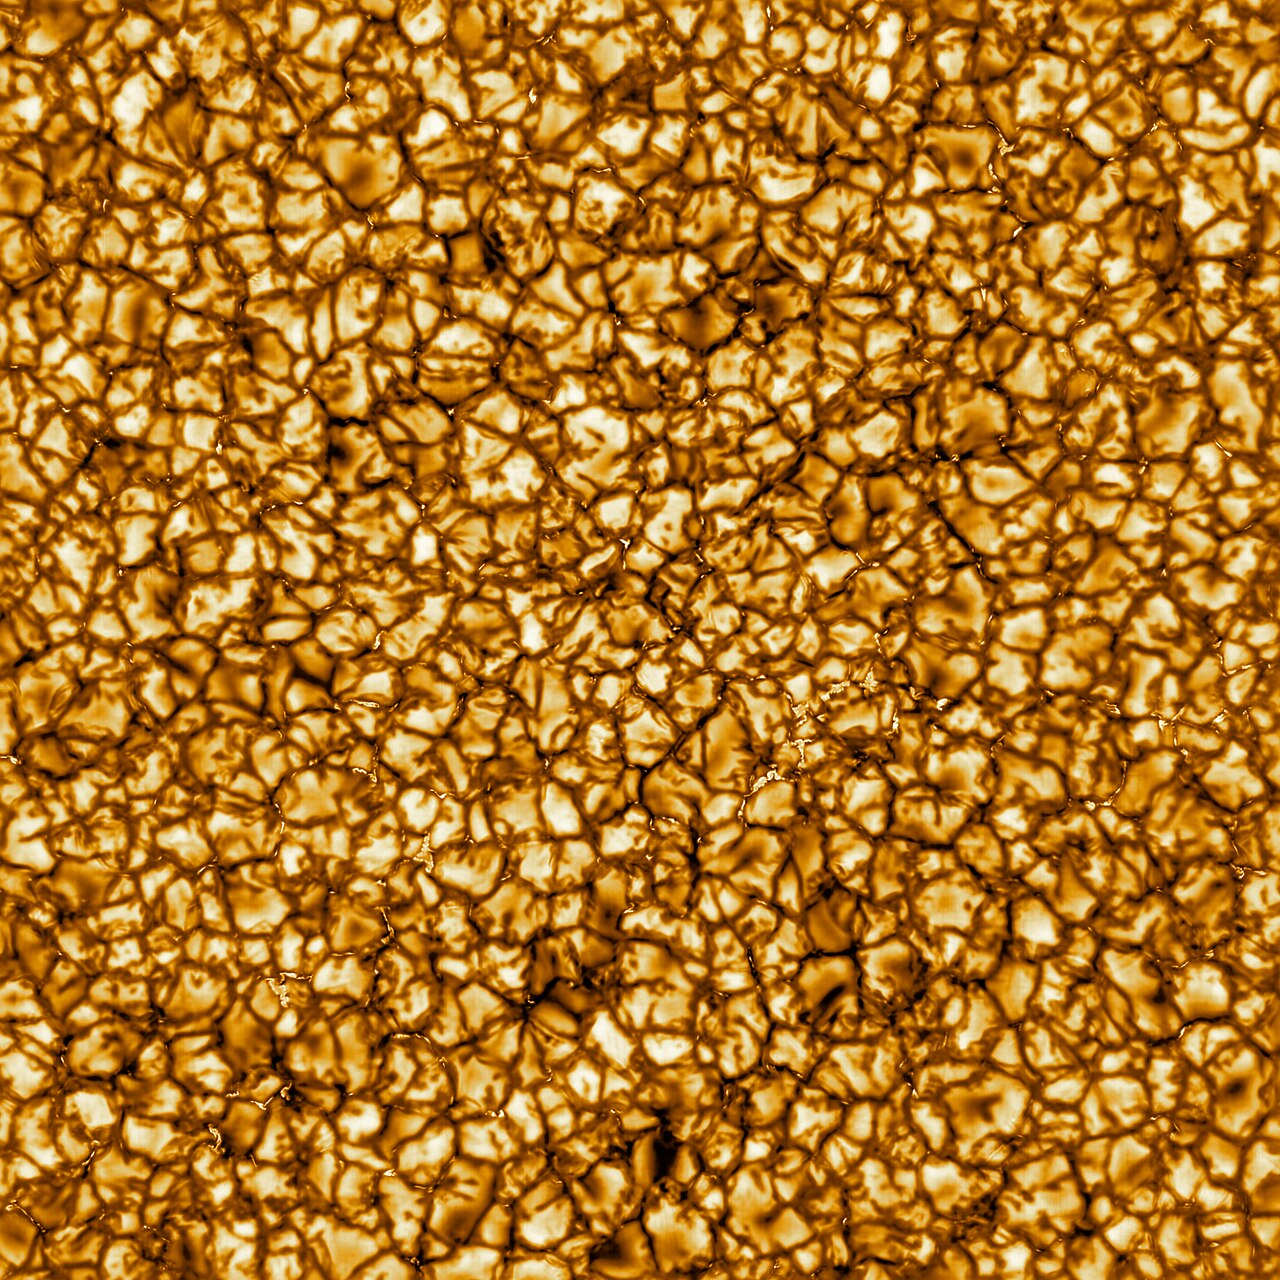
\includegraphics[width=100mm]{Images/Highest_resolution_photo_of_Sun_(NSF)_as_of_January_20,_2020.jpg}
        \caption{изображение ячеистых поверхностных структур Солнца.}
\end{figure}

Найдем температуру фотосферы. 
Будем считать Солнце АЧТ. Для рассчётов воспользуемся законом смещения Вина: 
\[
\lambda_{max} = \frac{0.29 }{T } \text{ см} \cdot \text{К}\Rightarrow T = \frac{0.29}{\lambda_{max}} \text{ см} \cdot \text{К},
\]
где $\lambda_{max}$ --- длина волны, при которой максимальна 
объёмная спектральная плотность излучения.  
\[
\rho_{\omega}(\omega, T)d\omega = \frac{\hbar \omega^{3}}{\pi^2 
c^3} \frac{d\omega}{e^{\frac{\hbar\omega}{k_{\text{Б}}T}} - 1} 
\]
\[
\rho_{\lambda}(\lambda, T)d\lambda = \frac{8\pi h c}{\lambda^5} \frac{d\lambda}{e^{\frac{h c}{k_{\text{Б}}T \lambda}} - 1}
\]

\newpage
\noindentИспользуя профиль регистограммы, найдем $\lambda_{max}$: 
\begin{figure}[H]
		\centering
		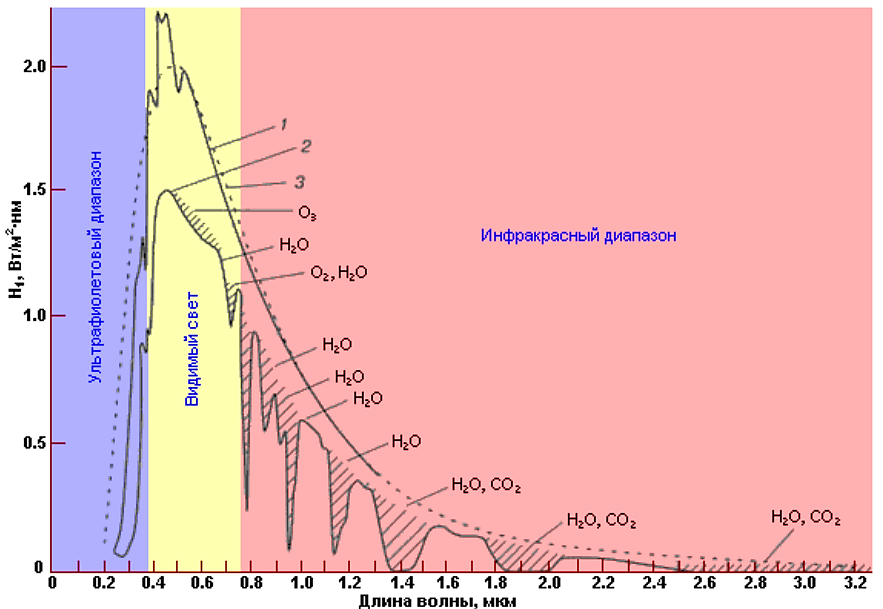
\includegraphics[width=170mm]{Images/Intensivity_.png}
        \caption{интенсивность падающего на Землю солнечного излучения в зависимости от длины волны: 1 --- солнечное излучение за границей атмосферы; 2 --- солнечное излучение на уровне моря; 3 --- излучение АЧТ при 5800 K.}
        
\end{figure}

\noindentДля \textbf{земной поверхности}: $\lambda_{max} = 0.47 \text{ мкм}\ \Rightarrow\ T \approx 6170$ К.\\

%\noindentЗа \textbf{пределами атмосферы}: $\lambda_{max} = 0.55 \text{ мкм}\ \Rightarrow\ T \approx 5273$ К.\\

\noindentДалее рассчитаем температуру фотосферы через закон Стефана-Больцмана:

\[
L = 4\pi R_{c}^2 \sigma T^4 \Rightarrow T = \left (\frac{L}{4 \pi R_{c}^2 \sigma}\right)^{\frac{1}{4}} \approx 5760 \text{ К, где } \sigma = 5,67 \cdot 10^{-8} \frac{\text{Вт}}{\text{м}^2\cdot\text{К}^4}
\]

\noindentПрименяя модель АЧТ для Земли, найдём температуру фотосферы:

\[
\sigma T^4 \cdot 4 \pi R_{\text{С}}^2 \cdot \frac{1}{4 \pi d^2} \cdot \pi R_{\text{З}}^2 = \sigma T_{\text{З}}^4 \cdot 4 \pi R_{\text{З}}^2\ \Rightarrow
\]

\[
T^4 \frac{R_{\text{С}}^2}{d^2} = T_{\text{З}}^4 \cdot 4\ \Rightarrow\
T = T_{\text{З}} \sqrt{\frac{2d}{R_{\text{С}}}} \approx 6218 \text{ К}.
\]

\noindentТабличное значение равно 6000 К.

\section*{Оценка температуры тёмных пятен}

\begin{figure}[H]
		\centering
		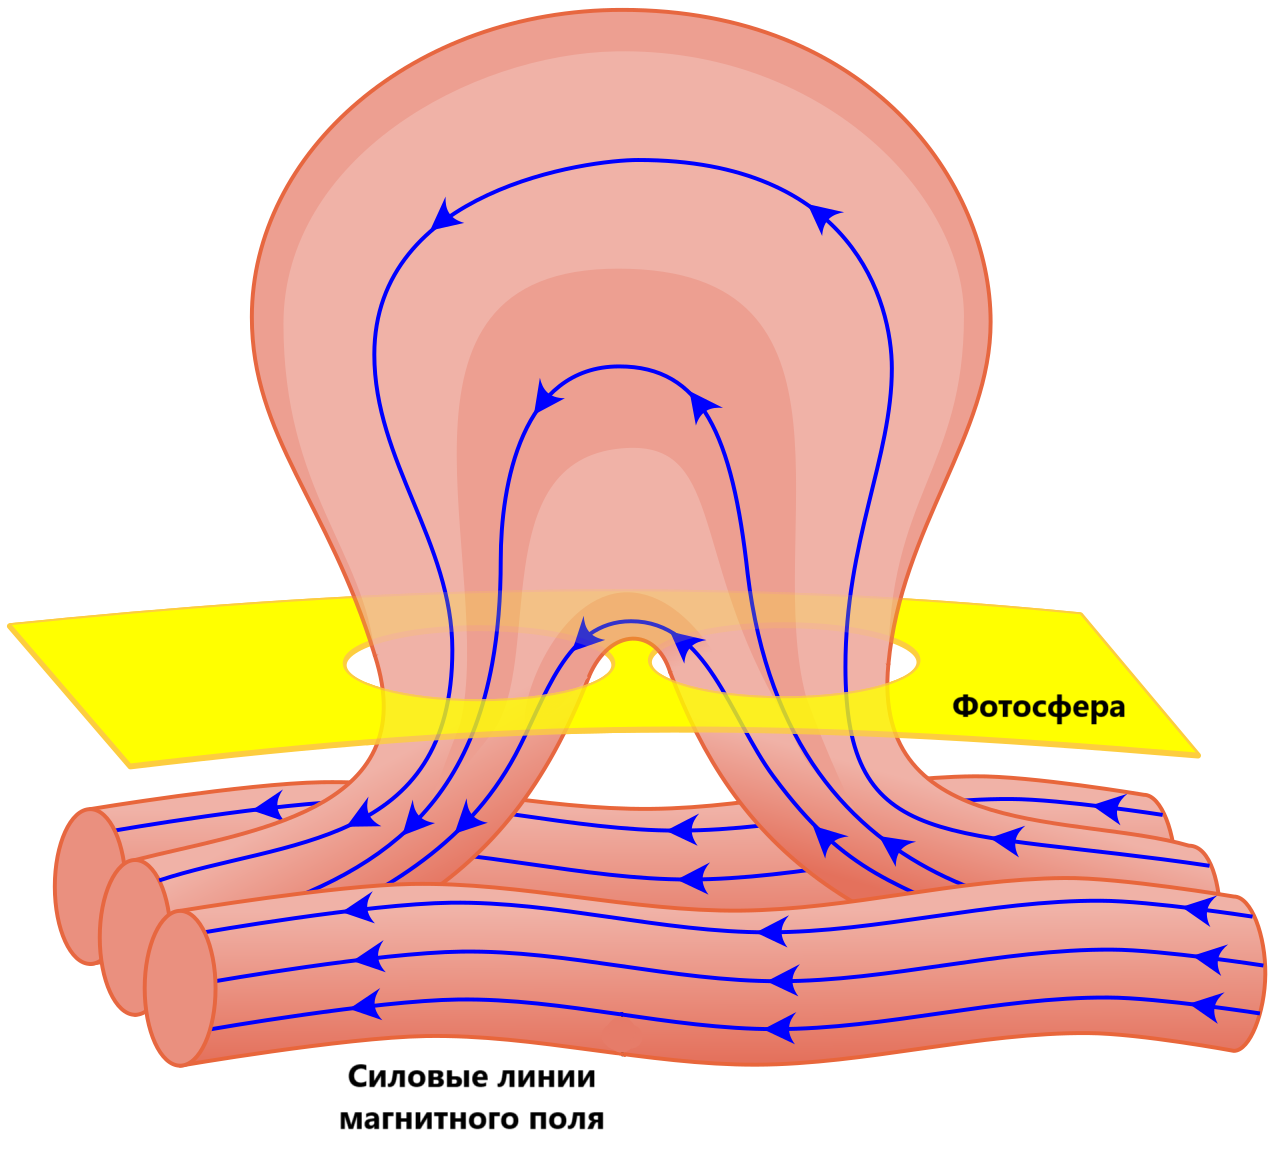
\includegraphics[width=100mm]{Images/Sunspot_diagram.svg.png}
        \caption{Принцип образования тёмных пятен на Солнце}
        
\end{figure}

На Солнце, а именно в фотосфере, наблюдаются тёмные пятна. Это тёмные области, температура которых ниже окружающих участков фотосферы. Солнечные пятна являются областями выхода в фотосферу отдельных участков сильных магнитных полей. Это объясняется тем, что вещество фотосферы представляет собой плазму, состоящую из заряженных частиц. Сильное магнитное поле тормозит движение плазмы и замедляет ее конвекцию из внутренних слоев Солнца. В результате температура вещества уменьшается. Температура тёмных областей на Солнце понижена примерно на 1500 К по сравнению с окружающими участками фотосферы.

Поток теплового излучения от Солнца однозначно связан с его температурой через закон Стефана-Больцмана. Яркость пятен составляет примерно 20---40\% от нормального света Солнца.
\[
\frac{T_{\text{С}}^4}{T_{\text{П}}^4} \approx \frac{1}{0.3}\ \Rightarrow\ T_{\text{П}} \approx T_{\text{С}} \cdot \sqrt[4]{0.3} \approx 4440 \text{ К}.
\]


\newpage
\section*{Оценка температуры ядра}

Попробуем оценить температуру сначала с \textbf{классической} точки зрения. Считаем протоны шариками с радиусами $r_p \approx 10^{-15}$ м. Тогда чтобы произошла ядерная реакция, нужно чтобы они сблизились на расстояние порядка $r_p$, чтобы сильное ядерное взаимодействие стало доминирующим. То есть кинетической энергии протонов должно хватить на преодоление кулоновского отталкивания:

\[
2\cdot\frac{m_pv^2}{2} = \frac{q^2}{r_p}, \text{ где } v^2 = \frac{3k_{\text{Б}}T}{m_p}. \text{ Тогда}
\]
\[
T = \frac{q^2}{3r_pk_{\text{Б}}} \approx 5.5\cdot 10^9\text{ K}
\]

Верна ли эта оценка температуры? Рассмотрим равновесие гравитационного притяжения и термодинамического давления самой плазмы в выделенном объёме. Приравняем все силы давления $P$, действующие каждый на достаточно маленький, чтобы считаться плоским элемент поверхности d$S$, окружающей выделенный объем $V$, и сумму сил притяжения каждого элемента массы d$m$, то есть: 
\[
\oint\limits_S PdS + \oint\limits_V \rho\nabla\varphi dV = 0
\]
По теореме Остроградского-Гаусса получим:
\[
\oint\limits_S PdS = \oint\limits_V \nabla PdV\ \Rightarrow\ \oint\limits_V (\nabla P + \rho\nabla\varphi)dV = 0
\]

Но поскольку мы никак не ограничивали выбор нашего объема, по которому ведется интегрирование, то единственный способ гарантировать выполнение этого условия --- потребовать, чтобы подынтегральное выражение было равно нулю в любой точке звезды. Тогда получается векторное дифференциальное уравнение, выражающее гидростатическое равновесие звезды:
\[
\nabla P = -\rho\nabla\varphi
\]

В случае, когда $\varphi = \frac{Gm(r)}{r} + C$, получим:
\[
\frac{dP}{dr} = -\frac{Gm(r)}{r^2}\rho
\]

Тогда для конечных приращений имеем:
\[
\frac{\Delta P}{\Delta r} = -\frac{GM_C\rho}{r^2}\ \Rightarrow\ P_C = \frac{GM_C\rho}{R_C}
\]

Давление идеального газа $P_C = \frac{\rho_Ck_{\text{Б}}T}{m_p}\ \Rightarrow\ \frac{M_C}{R_C} = \frac{2k_{\text{Б}}T}{Gm_p}$. Тогда при полученной температуре $T = 5.5\cdot 10^9\text{ K}$ имеем $\frac{M_C}{R_C} \approx 1.4\cdot10^{24}\ \frac{\text{кг}}{\text{м}}$. Но в действительности для Солнца $\frac{M_C}{R_C} \approx 2.9\cdot10^{21}\ \frac{\text{кг}}{\text{м}}$. Значит, оценка не верна, и классическая теория в данном случае неприменима!\\

Рассмотрим данный процесс с \textbf{квантовой} точки зрения. Протон
ведёт себя как волна и локализуется на расстоянии длины волны де Бройля:
\[
\lambda_p = \frac{h}{m_pv} = \frac{h}{m_p\sqrt{\frac{3k_{\text{Б}}T}{m_p}}} = \frac{h}{\sqrt{3k_{\text{Б}}Tm_p}}
\]
Тогда 
\[
2\cdot\left(\frac{3}{2}k_{\text{Б}}T\right) = \frac{q^2}{\lambda_p}\ \Rightarrow\ 3k_{\text{Б}}T = \frac{q^2}{\lambda_p}\ \Rightarrow\ T = \frac{q^2}{3k_{\text{Б}}\lambda_p} = \frac{q^2}{3k_{\text{Б}}}\cdot\frac{\sqrt{3k_{\text{Б}}Tm_p}}{h}
\]
Окончательно получаем:
\[
T = \frac{q^4m_p}{3k_{\text{Б}}h^2} \approx 4.88\cdot10^6\text{ K}.
\]

Снова оценивая данный результат с помощью гидростатического равновесия звезды, получаем $\frac{M_C}{R_C} = 2.43\cdot10^{21}\ \frac{\text{кг}}{\text{м}}$. Что по порядку величины совпадает с действительностью.\\\\

\section*{Оценка средней температуры Солнца}

Обозначим через $m(r)$ массу звездного вещества внутри сферы радиусом $r$, центр которой совпадает с центром звезды. При падении на эту сферу из бесконечности массы d$m$ выделяется гравитационная энергия $Gm\frac{dm}{r}$. Полная гравитационная энергия, освободившаяся при образовании звезды, выражается интегралом:
\[
G\int\limits_0^M\frac{m}{r}\ dm
\]

Половина этой энергии идет на нагревание звезды. В дальнейшем, когда гравитационное сжатие прекратится, внутри звезды должна выделяться энергия в результате термоядерных реакций, чтобы поддержать температуру и излучение звезды на неизменном уровне. В результате тепловая энергия звезды $К$ будет оставаться неизменной и выражаться половиной написанного выше интеграла. Этот интеграл можно было бы вычислить точно, если бы была известна плотность звездного вещества $\rho = \rho(r)$. Итак:
\hypertarget{1}
\[
\overline{K} = \frac{G}{2}\int\limits_0^M\frac{m}{r}\ dm = \frac{GM^2}{4}\left\langle\frac{1}{r}\right\rangle = \frac{GM^2}{4R}\left\langle\frac{R}{r}\right\rangle, \eqno(1)
\]
где $\left\langle\frac{R}{r}\right\rangle$ означает усредненное определенным
образом значение $\frac{R}{r}$, а именно:
\hypertarget{2}
\[
\left\langle\frac{R}{r}\right\rangle = \frac{2}{M^2}\int\limits_0^M \frac{R}{r}m\ dm \eqno(2)
\]
\\

Мы занимаемся оценкой средней температуры не звезды вообще, а звезды, только что образовавшейся из газово-пылевого облака, состоящего практически только из полностью ионизованного водорода. К этому времени водород еще не успел "выгореть"{} в результате термоядерных реакций. Из-за высокой температуры к нему применима классическая статистика Больцмана, которая и используется в дальнейшем.

Число протонов (а также электронов) в звезде составляет $\frac{M}{m_p}$, где $m_p$ --- масса протона. Поэтому тепловая энергия всей звезды равна $\frac{3Mk\overline{T}}{m_p}$.
Приравнивая её к выражению \hyperlink{1}{(1)}, получим:
\hypertarget{3}
\[
\overline{T} = \frac{GMm_p}{12kR}\left\langle\frac{R}{r}\right\rangle \eqno(3)
\]

Точное вычисление по формуле \hyperlink{3}{(3)} требует знания плотности вещества звезды $\rho$ в зависимости от расстояния $r$ до ее центра. Только тогда можно найти среднее значение отношения $\frac{R}{r}$. Но так как $\frac{R}{r} > 1$, то во всяком случае должно быть
\[
\overline{T} > \frac{GMm_p}{12kR}.
\]

Дополнительную работу можно частично учесть, если предположить, что конденсация ограничивается образованием звезды постоянной плотности $\rho$. В таком случае $T 
= \frac{4\pi}{3}\rho r^3,\ dm = 4\pi\rho r^2dr$ и формула \hyperlink{2}{(2)} дает $\frac{R}{r} = \frac{6}{5}$. В результате получается более точная, но все еще заниженная оценка средней температуры звезды:
\[
\overline{T} = \frac{GMm_p}{10kR}.
\]

Применим полученную оценку к Солнцу:
\[
\overline{T}_C \approx 2.3\cdot 10^6\text{ K}.
\]

Оптическим методам доступна температура только поверхности Солнца. Как мы убедились, она составляет около $6000$ К. Однако в современных моделях Солнца масса наружной оболочки, в которой температура меньше $10^6$ К, составляет всего около 1\% общей массы Солнца. Поэтому оболочка практически не сказывается на средней температуре Солнца.\\

Заметим, что мы получили практически $\overline{T}_C \approx T_{\text{ядра}}$, что не лишено смысла. По современной модели Солнца в сфере радиусом $r = \frac{R}{2}$ сосредоточено около 94\% полной массы. Если массой наружной оболочки пренебречь, то можно воспользоваться формулами выше, заменив в них радиус $R$ вдвое меньшей величиной. Тогда опуская расчёты, мы получили бы оценку вдвое больше для температуры солнечного ядра. Хотя, на самом деле концентрация вещества во внутренних зонах Солнца приводит к еще большему повышению температуры.

\newpage
\section*{Выводы}
\begin{enumerate}
    \item Солнце получает энергию из ядерных реакций, происходящих в его ядре.
    \item Произведена оценка температуры хромосферы по спектру поглощения 
$T_{\text{ср}} = $ 12 569 К, что согласуется с табличными данными (от 4000 К до 18 000 К).
    \item Произведены расчёты температуры фотосферы $T_{\text{С}} \approx 6218 \text{ К}$ (вне земной атмосферы), что согласуется с табличным значением 6000 К.
    \item Произведены расчёты температуры тёмных пятен, по предположениям составляющие примерно 20---40\% от нормального света Солнца. Получено значение $T_{\text{П}} \approx 4440 \text{ К}$, что согласуется с диапазоном табличных значений от 4000 К до 5500 К.
    \item Произведены расчёты температуры ядра Солнца  $T \approx 4.88 \cdot 10^6\text{ K}$, что по порядку величины сходится с табличным значением $T_{\text{С}} = 13.6 \cdot 10^6 \text{ К}$.
    \item Произведены расчёты средней температуры Солнца $\overline{T}_C \approx 2.3\cdot 10^6\text{ K, }$ что совпадает по порядку величины с температурой ядра $T\approx 4.88\cdot10^6\text{ K}.$
\end{enumerate}


\end{document}

https://en.wikipedia.org/wiki/Kelvin–Helmholtz_mechanism
https://ru.wikipedia.org/wiki/Протон-протонный_цикл
http://surl.li/gvdlnm
https://habr.com/ru/articles/405183/
https://www.wm.edu/as/physics/research/research_groups/high_energy_experiment/
https://en.wikipedia.org/wiki/Neutrino_oscillation#Theory
https://bass2000.obspm.fr/solar_spect.php
https://www.nuclear-power.com/glossary/doppler-broadening/
https://nplus1.ru/blog/2018/04/27/sunny
